% !TEX encoding = UTF-8
% !TEX TS-program = pdflatex
% !TEX root = ../tesi.tex

\begin{usecase}{4}{Visualizzazione Dati ordinati per Procedimenti}
  \usecaseactors{Utente autorizzato}
  \usecasepre{L'utente si trova all'interno dell'applicazione}
  \usecasedesc{Permette la visualizzazione dei dati caricati da CD}
  \usecasepost{L'utente può visualizzare i dati caricati da CD ordinati per procedimenti}
  \label{uc:visualizzazione-dati-procedimenti}
\end{usecase}


\subsection{UC4 - Visualizzazione dati ordinati per procedimenti}
\begin{itemize}
  \item \textbf{Identificativo}: UC4
  \item \textbf{Nome}: visualizzazione dati ordinati per procedimenti
  \item \textbf{Descrizione grafica}:
\end{itemize}

\begin{figure}[h]
  \centering
  %  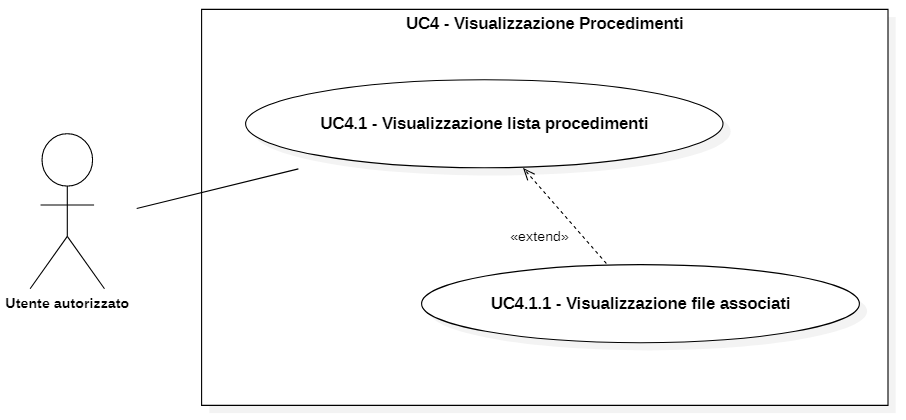
\includegraphics[scale=0.50]{images/UC4.png}
  \caption{Descrizione grafica caso d'uso UC4}
\end{figure}

\begin{itemize}
  \item \textbf{Attori}
        \begin{itemize}
          \item \textit{Primari}: utente autorizzato
        \end{itemize}
  \item \textbf{Precondizione}: l'utente si trova sulla pagina per il caricamento dati, che ha già effettuato correttamente.
  \item \textbf{Postcondizione}: l'utente visualizza i dati caricati sull'applicazione, ordinati per procedimenti.
  \item \textbf{Scenario principale}: l'utente ha caricato correttamente i dati e questi vengono visualizzati ordinati per procedimenti.
\end{itemize}
\newpage